\section{FPGA}
FPGA'en fungerer som en del af den hardware der styrer pan/tilt-systemet. FPGA'ens opgaver er bl.a. dataopsamling fra hall sensorene på motorerne, sende styre signaler til H-broerne, genererer pwm signaler, implementerer en form for sikkerhedsbegrænsning på hvor meget pan og tilt kan dreje rundt samt at kommunikerer med MPU'en. Afsnittet er delt op i separate beskrivelse af de moduler som FPGA'en er bygget op af. \\

\subsection{SPI}
Der skal foregå en kommunikation mellem microcontrolleren og FPGA'en. Til dette formål er der i opgaven specificieret at grænsefladen SPI skal bruges. Grænsefladens overordnede virkemåde er beskrevet nærmere i afsnit \ref{subsec:SPI}. Microcontrolleren fungerer som master i denne kommunikation. I dette afsnit vil der blive beskrevet fordele og ulemper ved forskellige måder at implementerer denne grænseflade i FPGA'en. Dernæst vil der blive foretaget en dybere gennemgang af den valgte implementation. Og konkluderes på, hvordan denne implementation har fungeret rent praktisk.

\subsubsection{Kommunikation med MPU}
Kommunikationen fra FPGA'en til MPU'en foregår over SPI, men da SPI kun er en grænseflade. Skal der defineres, hvordan de datapakker der sendes frem og tilbage tolkes. Til at gøre dette er det blevet overvejet to forskellige metoder som er beskrevet i de følgende afsnit.

\paragraph*{8-bit pakker med kommunikationsprotokol}
Dette var den første implementation der blev overvejet. Her sendes data mellem FPGA og MPU i pakker af størrelsen 8-bit. Der skal så fastsættes en kommunikationsprotokol der består af telegrammer med et vidst antal bytes i. Og i hver ende skal der være en controller der kan afkode de telegrammer der kommer ind. Og ud fra det bestemme hvad der skal foretages i FPGA'en. Fordelen ved denne implementation er at alt afhængig af hvordan telegrammerne designes så kan der både implementeres crc-check af beskederne og en masse kommandoer. Ulempen er at man skal opstille en protokol for kommunikationen og at der skal overføres flere pakker før at der reelt set sker noget samt at selve kommunikationen bliver mere kompliceret.

\paragraph*{16-bit pakker med 4-bit addressering}
Denne implementering involverer at man bruger 16-bit per overførsel. De øverste 4-bit bliver brugt til at addresserer, hvilket modul inde i FPGA'en der ønskes kommunikation med. Og de resterende 12-bit kan bruges til at overfører data med. En 4-bit addresser giver mulighed for at kunne addresserer op til 16 moduler i FPGA'en.

\subsubsection{Kommunikation internt med moduler}
Når datapakkerne fra SPI er modtaget i FPGA'en skal de på en eller anden måde tolkes. Og ud fra denne tolkning skal der enten sendes data til et modul eller hentes data fra et modul. Her beskrives de to måder der er blevet overvejet til at håndterer den interne kommunikation mellem FPGA'ens moduler.

\paragraph*{Master Controller}
Ved denne måde at kommunikerer på skal der internt i FPGA'en opbygges et "master" modul der har forbindelse til alle de forskellige andre moduler igennem individuelle busser. På den måde vil der aldrig kunne opstå data kollisioner pga. at flere moduler forsøger at sende data på samme tid. Master modulet vil så altid have alt data fra alle moduler tilgængeligt, men det vil i sidste ende give voldsomt mange forbindelser som det kan ses på figur \ref{fig:FPGA_MasterController}. Da der skal være en bus per signal. Master controlleren skal også stå for at afkode det der kommer fra SPI og sende/sætte det rigtige data i de andre moduler. Så denne bliver meget kompleks og ikke særlig modulær idet at der skal ændres en hel del når der sker en ændring i modulerne.

\begin{figure}[ht]
	\begin{center}
		\includegraphics[scale=0.75]{Billeder/FPGA_MasterController.png}
	\end{center}
\caption{Grafisk afbilding af et system, hvor de interne moduler alle er koblet til et master modul. Her modtages data fra MPU'en via en 8-bit protokol der afkoder hvilket modul der skal kommunikeres med}
\label{fig:FPGA_MasterController}
\end{figure}

\paragraph*{Databus og addressering}
Ved at have en intern data- og addresse-bus kan alle modulerne kobles op på den samme databus. For at der ikke opstår data sammenstød fordi to moduler forsøger at skrive til bussen, bliver der også nødt til at være en form for kontrol af hvornår der må skrives til bussen. Denne kontrol udføres ved hjælp af en addresse. Modulerne tilgår kun databusen når det er deres addresse der står på addressebussen samt et read/write signal der styrer, hvornår et modul må skrive til bussen og hvornår det data der står på bussen er klar til at blive læst. For nemmest at implementerer dette indføres der et modul som agerer master og som er den eneste enhed der kan bestemme, hvad der står på addressebussen, samt hvilken tilstand read/write signalet er sat til. En grafisk afbilding af dette kan ses på figur \ref{fig:FPGA_Databus}.

\begin{figure}[ht]
	\begin{center}
		\includegraphics[scale=0.75]{Billeder/FPGA_Databus.png}
	\end{center}
\caption{Grafisk afbildning af et system, hvor de interne moduler sidder på en fælles databus med styring af denne via en addressebus og et read/write signal. Og addressering sker direkte via de modtagne 16-bit fra SPI}
\label{fig:FPGA_Databus}
\end{figure}

\paragraph*{Implementering}
SPI modulet er blevet implementeret som en løsning bestående af en 16-bit grænseflade til MPU'en. Og en intern databus, hvorpå modulerene addresseres direkte igennem de øverste 4 bit i SPI datagrammet. SPI modulet fungerer ved en tilstandsmaskine som er vist på figur \ref{fig:FPGA_SPI_State} og de forskellige tilstande er som følgende:\\
SPI starter i tilstanden \textit{WaitForSSLow}, hvor der ventes på at SS signalet går lavt og kommunikationen derved er startet. Når SS går lavt skiftes der til tilstanden \textit{WaitForAdr}. \\ 
I denne tilstand ventes der på at MPU'en overfører de fire første bit i datagrammet, som repræsenterer addressen på det ønskede interne modul, og sender disse ud på addressebussen. Når de er modtaget skiftes der til tilstanden \textit{LoadUdBuf} \\
I denne tilstand loades data fra databussen ind i udbufferet så de er klar til at blive sendt afsted når MPU'en clocker SPI igen.\\
Dernæst skiftes der til tilstanden \textit{WaitForDatabits}. \\
I denne tilstand ventes der på at MPU'en clocker de sidste 12 databits ud. Når disse er modtaget skiftes der til tilstanden \textit{WE0}, hvor WE sættes til nul, hvilket fortæller det addresserede modul at det kan læse gyldig data ind fra databussen. \\ Derefter skiftes der til tilstanden \textit{WaitForSSHigh}, hvor WE sættes høj igen så modulerne ikke længere læser på databussen. Og der ventes på at SS sættes høj igen og datatransmissionen derved er slut. Så skiftes der til tilstanden \textit{WaitForSSLow} og det hele kører forfra igen.

\begin{figure}[ht]
	\begin{center}
		\includegraphics[scale=0.5]{Billeder/FPGA_SPI_State.png}
	\end{center}
\caption{State machine diagram over de states som SPI modulet går igennem}
\label{fig:FPGA_SPI_State}
\end{figure}

\subsection{PWM Driver}

PWM driveren har til opgave at levere et PWM-signal, med en duty cycle bestemt af et input fra microcontrolleren. Denne sektion vil beskrive designet af driveren samt nogle af de bevæggrunde der har ligget bag valget af dette design.

\subsubsection{Designmål}

\begin{itemize}

\item PWM frekvens mellem 20 kHz og 25 kHz
\item 8 bits PWM opløsning
\item Inputtet skal latches før duty cycle ændres

\end{itemize}

\subsubsection{Inputs}

Hovedårsagen til at der bliver brugt et 8 bits input til at vælge duty cycle, er at denne størrelse tit bliver brugt i microcontrollere, da arkitekturen er bygget op omkring data i forskellige byte-størrelser. Denne begrænsning findes som sådan ikke på en FPGA, da man selv kan lave sin arkitektur som man vil. Men hvis man formindsker bitstørrelsen for effektivitetens skyld, formindsker man også opløsningen for den duty cycle man kan vælge, og det er måske ikke hensigtsmæssigt i et kontrolsystem. Som udgangspunkt virker en opløsning på 8 bit som et fint kompromis XXXX.

Driveren har også brug for et clock-signal til at regulere timingen i den samt et latching input. Dette input lader PWM-modulet læse værdien af input-bus'en ind i driveren's egen hukommelse og derved ændre duty cycle.

\subsubsection{PWM Frekvens}

Der er en række ting man skal være opmærksom på, når man vælger frekvensen pulserne skal sendes ved. Jo højere frekvensen er, jo mere tid tilbringer man i switching transistoren's aktive område - det vil sammenlagt give et større effekttab. Frekvensen er til gengæld også nødt til at være høj nok til at motoren's inerti kan glatte de elektriske pulser ud rent mekanisk. Derudover er det også nemmere for motorspolerne at holde strømmen nogenlunde konstant ved en højere frekvens - det er blandt andet en af antagelserne fra den matematiske motormodel. Der skal også tages højde for de vibrationer, der genereres når motorinputtet kommer i pulser. Hvis frekvensen er mindre end 20 kHz, ligger vibrationerne inden for det hørbare område for mennesker, og det er ikke altid hensigtsmæssigt. Motoren og ophængets egenfrekvens skal også undgås - denne frekvens vil være højere jo mere stift ophæng motoren har, men den vil typisk ikke ligge i det supersoniske område. Alle disse ting peger tilsammen imod en PWM frekvens på den anden side af 20 kHz, men ikke meget derover. 

Med et 8 bits input skal hver pulsperiode deles ind i 256 lige store dele (se ligning \ref{eq:pwm_slice}, hvor $T_{slice}$ er bredden i $\mu s$), så det er muligt at flytte tidspunktet, hvor der skiftes fra høj til lav og dermed få en anden duty cycle. 

\begin{equation}\label{eq:pwm_period}
T_{PWM}=\dfrac{1}{25 kHz} = 40 \mu s
\end{equation}

\begin{equation}\label{eq:pwm_slice}
T_{slice}=\dfrac{T_{PWM}}{256}=156ns
\end{equation}

En clock-periode med FPGA'ens krystal på 50 MHz er $20ns$ lang, så hvis man tæller en variabel op hver 8. clock-periode til den når 256, så får man en samlet periodetid på $20ns*8*256=40.96 \mu s=24.414kHz$. Denne variabel sammenlignes så med den lagrede 8 bits duty cycle værdi, for at afgøre om signalet på udgangen skal være højt eller lavt. På figur \ref{fig:PWM_timing} kan man se en grafisk repræsentation af modulets virkemåde.

\begin{figure}[ht]
	\begin{center}
		\includegraphics[scale=0.5]{Billeder/PWM_Timing.png}
	\end{center}
\caption{Ramperne på den øverste graf repræsenterer variablen der tælles op fra 0 til 255. På den nederste graf ses det resulterende PWM-signal}
\label{fig:PWM_timing}
\end{figure}

\subsection{Positions modul}
\label{subsec:TicksToDeg}

For at kunne ramme et punkt på himlen, bliver microcontrolleren nødt til at vide hvilken position pan-tilt systemet står i.
For at kende denne position, er der to hall sensorer på EMG30 motoren.
Disse sensorer sidder 90 grader forskudt, når motoren har kørt en omgang (Den indre rotor) har hall sensorerne sendt høj 3 gange hver.
Hver gang en hall sensor går fra høj til lav, eller lav til høj, vil et register i FPGA'en inkrementere et register med 1.\\

For at kunne finde ud af hvilken vej motoren kører, kigges der på hvordan hall sensorerne går høj og lav i forhold til hinanden.

\begin{figure}[ht]
	\begin{center}
		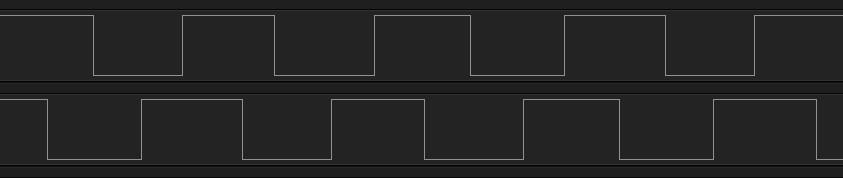
\includegraphics[scale=0.5]{Billeder/Hall_sensorer.png}
	\end{center}
\label{fig:Hall_Sensorer}
\caption{Her ses et billede af hvordan hall sensorerne går høj og lav i forhold til hinanden}
\end{figure}

Rotation.
Når hall sensor 1 er høj, og hall sensor 2 er høj\\
Hvis så hall sensor 2 bliver lav først, så er det en rotation med uret.\\
Og hvis hall sensor 1 bliver lav først, så er det mod uret.\\

Når hall sensor 1 er lav, og hall sensor 2 er lav\\
Hvis hall sensor 2 så bliver høj først, så er det en rotation med uret.\\
Hvis hall sensor 1 bliver høj først, så er det en rotation mod uret.\\

\subsection{MotorController}
Motor Controller har til formål at styrer en motor. Modulet skal kunne starte og stoppe motoren, styrer retningen af motoren, styrer hastigheden af motoren samt implementerer en sikkerhed så motoren ikke ødelægger pan delen af systemet, hvis der kommer forkert input til motorcontrolleren.

\subsubsection{Designmål}
Liste over ting som motorcontrollen skal kunne:
\begin{itemize}
	\item Være generisk så dens parametre kan tweakes til flere motorer
	\item Slå motorbremsen til og fra.
	\item Skifte retning på motoren
	\item Kunne stoppe motoren fra at drive pan- og til-rammerne ud over deres fysiske begrænsninger.
\end{itemize}

\subsubsection{Implementation}
Motor controlleren tager et input fra den fælles interne databus og har en addresse tildelt der er generisk, så der er mulighed for at ændre denne. Der er også forbindelse til en knap som kan sbruges til at styrerer modulet. Modulet er implementeret som en tilstandsmaskine som vist på figur \ref{fig:FPGA_MotorController_State} og er beskrevet som følgende:\\
\textit{Idle} dette er den tilstand som systemet starter i. Her sørges der for at motoren ikke kører. Der ventes på at knappen bliver trykket ned. Når dette sker skiftes der til tilstanden \textit{ZeroRelease}.\\
I denne tilstand ventes der på at knappen bliver sluppet igen for at undgå at inputet fra knappen overføres til næste tilstand. Når knappen bliver sluppet skiftes tilstanden til \textit{ZeroMotor}.\\ 
I denne tilstand er det muligt at nulstille motorens position ved hjælp af knappen. Når knappen trykkes ned så kører motoren i en retning og når knappen slippes og trykkes igen så kører motoren den anden retning. Dette fortsætter indtil at modulet registrer at der er gået forbi index hall sensoren. Når dette sker så signaleres andre moduler om at motoren er færdig med at nulstille og tilstanden skifter til \textit{PostZero}.\\
Denne tilstand er til for at det er muligt at vælge, hvornår at FPGA'en overlader kontrollen af motorerne til det der kommer ind fra databussen. Der ventes på at knappen trykkes ned og når dette sker så skiftes der til tilstanden \textit{RunMode}. \\
I denne tilstand så styres motoren af det der kommer ind til modulet via den interne databus. Der tjekkes hele tiden på om motorens position går ud over de grænser som der er defineret den skal holde sig inden for. Hvis der bliver gået ud over disse grænser ændres så skiftes tilstanden til \textit{EmergencyMode}.\\
I denne tilstand slår modulet motorbremsen til og låser motorerne fast. Efterfølgende input fra databussen ignoreres og der ventes på at knappen bliver trykket ned. Når dette sker så skiftes tilstanden tilbage til \textit{Init} og motoren skal nulstilles på ny.

\begin{figure}[ht]
	\begin{center}
		\includegraphics[scale=0.5]{Billeder/FPGA_Motorcontroller_state.png}
	\end{center}
\caption{State machine diagram over de states som MotorController modulet går igennem}
\label{fig:FPGA_MotorController_State}
\end{figure}

\subsection{Diverse undermoduler}
Her beskrives diverse små undermoduler der ikke er store nok til at have en sektion for sig selv, men som stadigvæk tilføjer mindre funktionaliteter til FPGA'en.

\subsubsection{NumberToBCD}

Lad os først definerer BCD. BCD, eller Binary Coded Decimal, er et format hvor hver decimal ciffer er beskrevet ved et 4 ciffer binært tal. 1234 vil således være 0001 0010 0011 0100.
\\
Det er meget brugbart at benytte nettop denne notation til at give decimal tal videre mellem moduler. Dette bliver brugt til MultiplexDisplayet, som nettop skal displaye decimal tal, og derfor har brug for at tallene bliver lavet om fra de binære tal der arbejdes med til noget der kan repræsenterer hvert display enkeltvis.
\\
Måden dette gøres på er ved brug af en algorithme. Denne fungerer således:

\begin{enumerate}
\item Hvis et tal i en kolonne er større end 4 lægges der 3 til.
\item Logical shift left
\item Hvis der er foretaget $3 \cdot n - 1$ skift, hvor n er antal kollonner, så afsluttes der
\item Gå til 1.
\end{enumerate}

\subsubsection{MultiplexDisplay}

MultiplexDisplayet har to primære funktioner. Den ene, og ironisk nok den vigtigeste, er ikke display funktionalitet, men i stedet clock scaling. Denne fungerer ved at tage det indbyggede clock signal med en frekvens på $50 MHz$ og skalere det ned til $1 kHz$. Dette sendes ud som et signal til alle de andre moduler, så det er sikret at hele FPGA'en er synkroniseret, så meget som det nu er muligt.
\\
Den anden funktionalitet er så at tage et input i from af BCD kode og lave det om til de tilsvarende display karakterer. Da displayet fungerer ved at man outputter en enkelt karaktere ad gangen skiftes der mellem de fire displays, og dermed også de fire dele som inputtet er indelt i.

\subsubsection{ToggleButton}

Ved hver af de brugte knapper er der et modul der holder styr på outputtet af knappen, og inddelere det i tre forskellige signaler.

\begin{itemize}
\item Pulse
\item Debounce
\item Toggle
\end{itemize}

Disse er implementeret i form af en state machine der benytter et fire bit shift register der afhænger af input til at ændre tilstand. Når knappen bliver trykket ned i fire clock pulser i træk skifter state machinen over i den tilstand der svarer til at alle output er tændt. Puls signalet bliver slukket næste clock puls, mens debounce signalet bliver slukket når knappen ikke har været trykket ned i fire signaler i træk. Toggle signalet bliver selvsigende slukket næste gang der bliver trykket på knappen i fire clock signaler i træk, hvor pulse og debounce naturligvis også bliver aktiveret.

\subsection{Endeligt design}
Når man kigger på, hvilke behov der er i forhold til kommunikation med FPGA'en så kan det ses at der kun foregår dataudvekslinger mellemm FPGA og MPU dvs. at MPU'en enten henter en værdi ud af FPGA'en eller sætter en værdi i denne. Der er derfor ikke behov for en protokol der kan tage imod deciderede kommandoer og udfører komplekse ting i FPGA'en, men nærmere behov for at der hurtigt kan sættes/hentes en værdi. Hele SPI interfacet skal kun fungerer som en udvidelses af den funktionalitet der allerede ligger i MPU'en dvs. at der skrives til et register for at få en enhed til at gøre noget eller læses fra et register for at få en værdi ud af en enhed. På den måde behøver grænsefladen set fra MPU'ens side ikke være særligt avanceret. Ved at kigge på dette behov blev det besluttet at et 16-bit datagram format, hvor de første 4 bit angiver en addresse på et modul, ville være tilstrækkeligt. Da FPGA'en kører med en clockfrekvens på 50MHz og SPI clocken vil kører væsentligt langsommere. Så er det muligt at implementerer protokollen således at data kan hentes fra FPGA'en, i samme datagram udveksling som addressen på det modul dataen skal hentes ud fra bliver modtaget. Da der både bliver clocked data ud fra MPU'en samtidig med at data bliver clocked ind fra FPGA'en. Så skal FPGA'en sende addressen ud når de første 4 bit er modtaget og sætte et write signal som tillader det modul der har addressen at sende sin data ud på databussen.\\
I selve FPGA'en er det blevet valgt at implementerer to databusser. En til data der kommer fra moduler og skal ud på SPI. Og en til data der kommer fra SPI og skal ind til et modul. Dette er gjort fot at undgå at bruge et INOUT signal internt i FPGA'en da der ikke forefindes hardware til at tristatte interne signaler. Så i sidste ende får man warnings i Xilinx og det bliver lavet om til logiske kredse som har nogenlunde samme funktionalitet, men så kan man ligeså godt designe det sådan til at starte med.\\
Der eksisterer et sæt motorcontroller og positionsmodul til hver motor. Disse moduler har forskellige addresser og fungerer som seperate enheder. De har også hver deres grænser defineret for motoren da pan og tilt ikke har samme grader af bevægelsesfrihed.\\
Af extra features er der implementeret sådan så at det er muligt altid at se hvilken position pan eller til står i. Da dette vises på de fire syvsegment-displays der sidder på udviklingsboardet. Det er muligt at skifte mellem hvilken værdi der vises på displayet ved at skifte på en kontakt på boardet. Hele implementeringen af FPGA'en kan ses som et blokdiagram på figur \ref{fig:FPGA_Final}.

\begin{figure}[ht]
	\begin{center}
		\includegraphics[scale=0.5]{Billeder/FPGA_Final.png}
	\end{center}
\caption{Blok diagram over modulerne i FPGA'en. Eksterne inputs er røde. Interne signaler er sorte. Eksterne outputs er gule. Databussen er lilla. Interne moduler er grå. Intern logic er lilla. Ekstern enhed er grøn}
\label{fig:FPGA_Final}
\end{figure}